\documentclass{article}

\usepackage{graphicx}
\usepackage[colorlinks=true]{hyperref}
\usepackage[format=plain, labelfont=it, font=footnotesize, labelsep=period]{caption}
\usepackage[margin=1in]{geometry}
\usepackage{amsmath}
\usepackage{amssymb}

\renewcommand{\theequation}{\arabic{section}.\arabic{equation}}

\begin{document}

\begin{titlepage}
\vspace*{\stretch{1}}
\centering
\Huge Investigating the Mathematics behind Edge Detection
\vspace*{\stretch{1}}
\end{titlepage}

\tableofcontents
\newpage
\listoffigures

\newpage

\section{Introduction}
As a programmer and hobbyist graphic designer, I have worked with many vector and raster-based design programs ranging from Gravit Designer to Adobe Photoshop, and wondered about how certain features are implemented. Thus, I focused my attention to the mathematics governing algorithms used in 2D computer graphics, but my initial stages of research revealed many areas that could be potentially explored. However, I remember one day I tried to vectorize a photograph by tracing around it with the pen tool, which sparked my desire to explore how a computer would “trace” a photograph through edge detection.

\begin{figure}[!hbtp]
    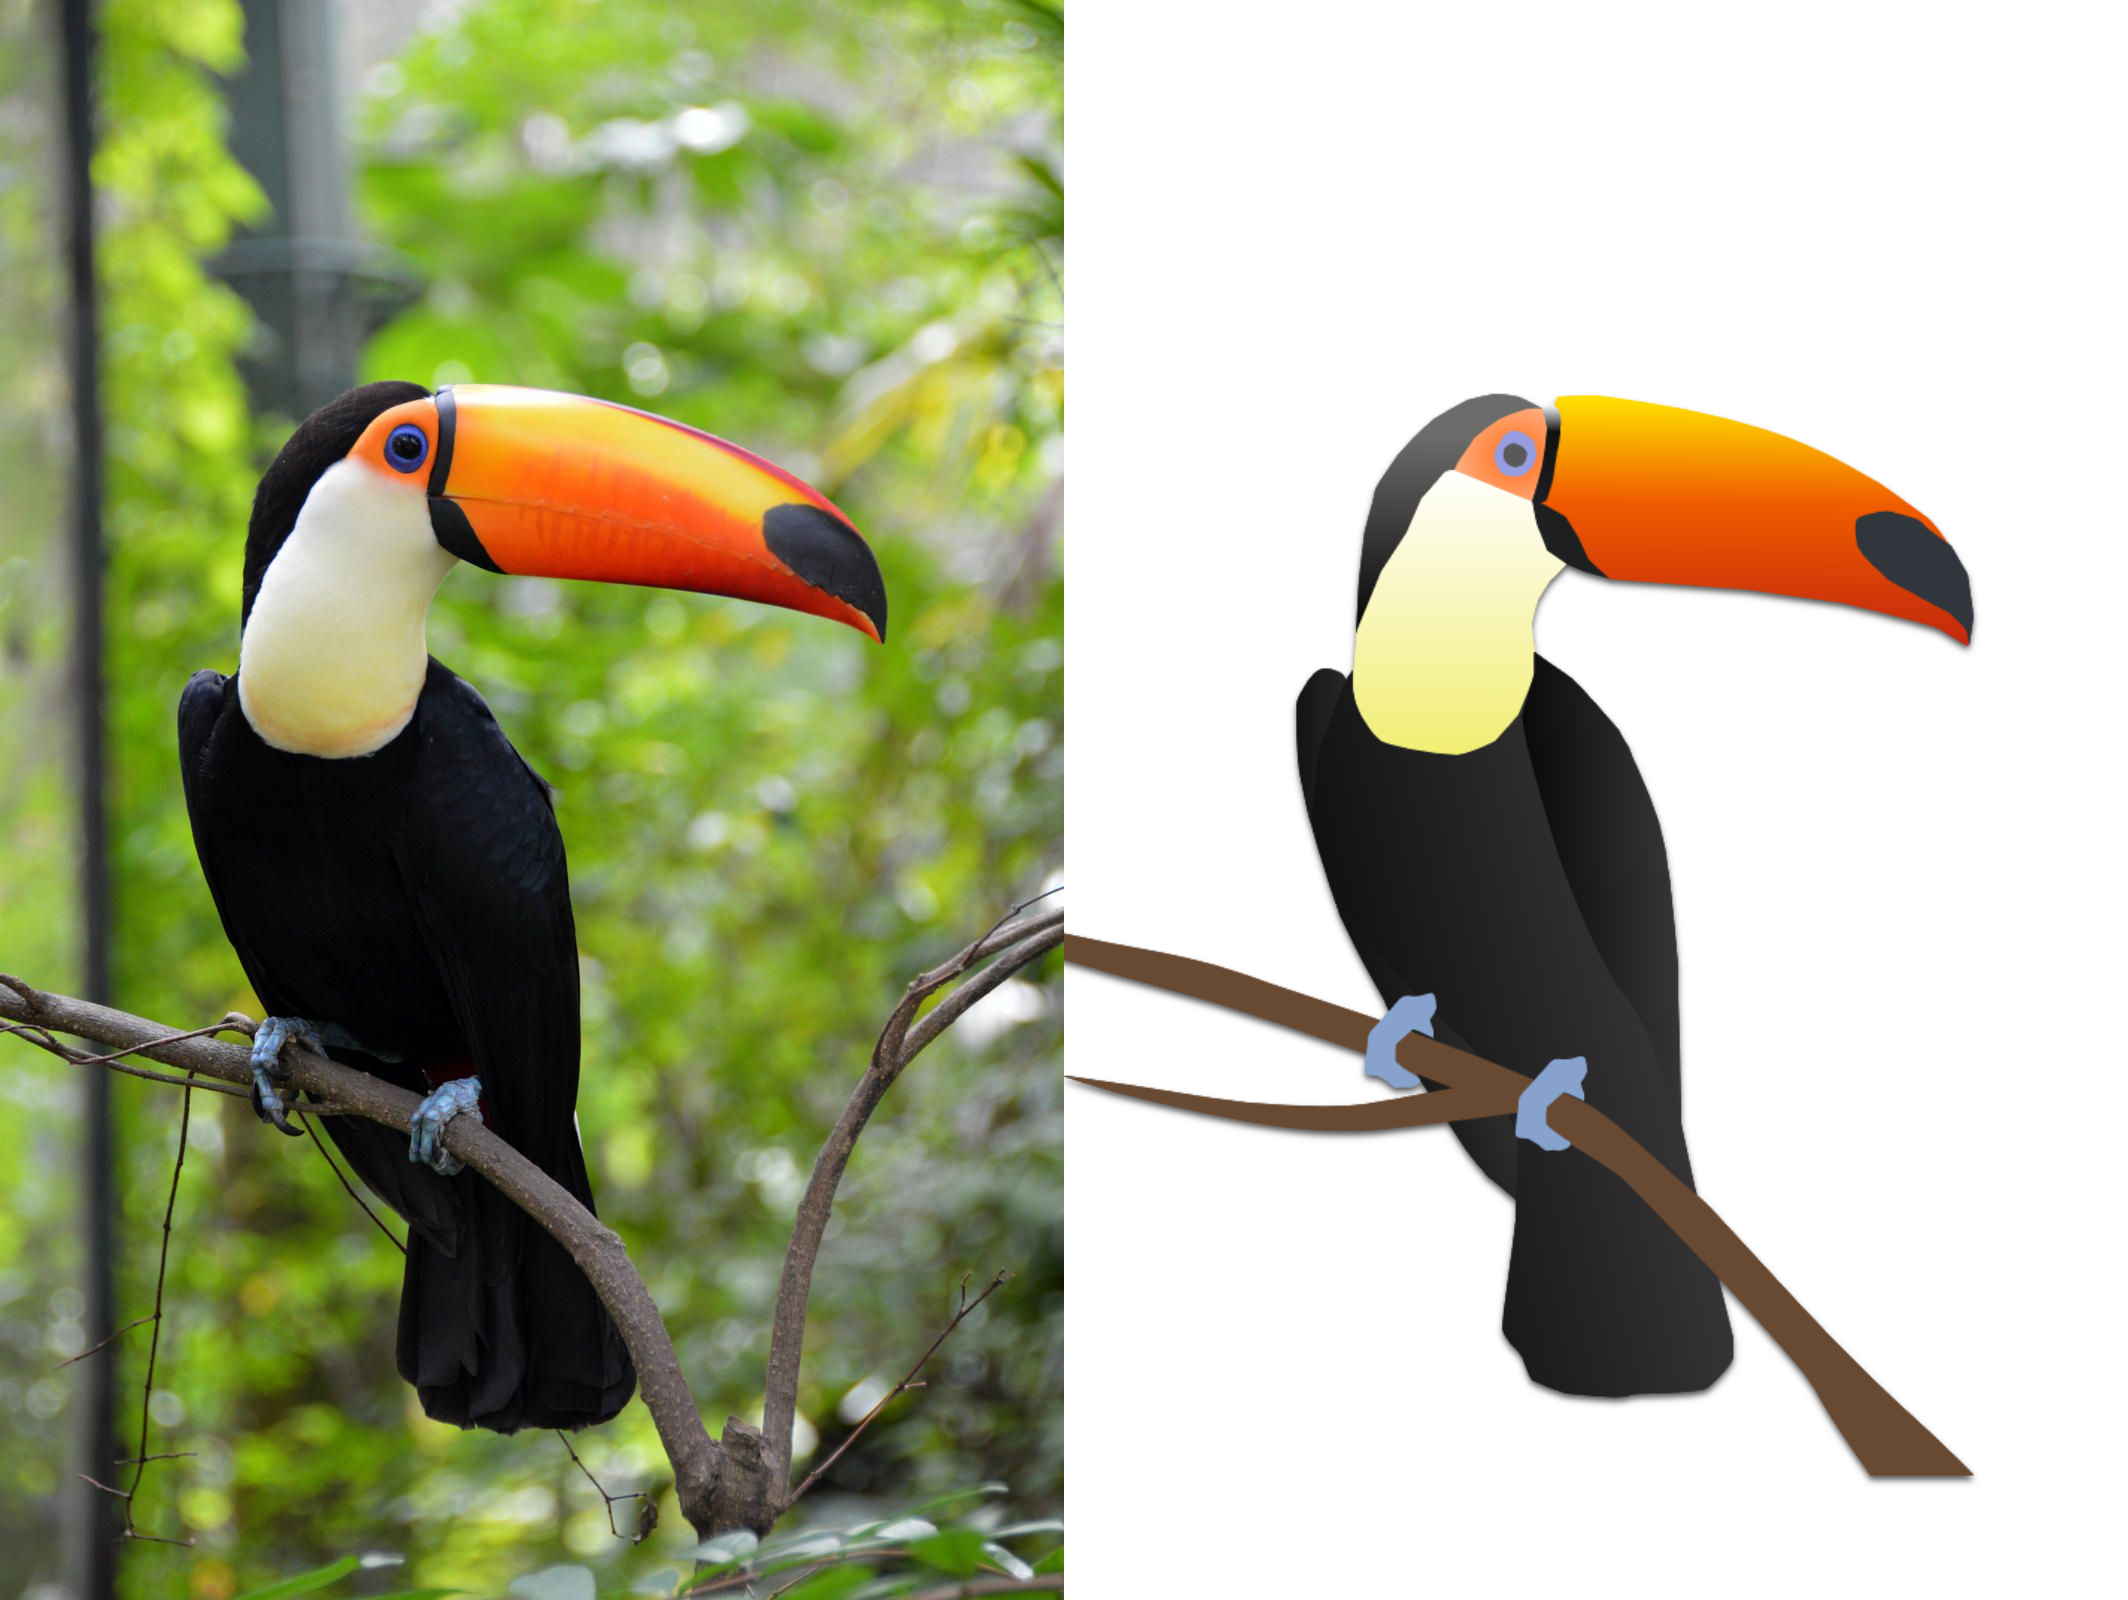
\includegraphics[width=\textwidth]{figures/figure01.png}
    \caption[The exact image I tried to trace]{\centering The exact image I tried to trace. Left image retrieved from \href{https://static.wikia.nocookie.net/maker-scratchpad-youtube/images/2/2a/Toco_Toucan.jpg/revision/latest?cb=20200318045659}{https:\slash\slash static.wikia.nocookie.net\slash maker-scratchpad-youtube\slash images\slash 2\slash 2a\slash Toco\_Toucan.jpg\slash revision\slash latest?cb=20200318045659}}
    \label{fig:The exact image I tried to trace}
\end{figure}

Otherwise specified, all images used for this maths exploration were taken or generated by me. Additionally, code used to generate some of these images can be found in the appendix. When coding, I tired to stay as far as possible from using external libraries that provided implementations for algorithms performed on images. This allowed me to thoroughly demonstrate my understanding of the mathematics involved in the concepts that will be discussed in my exploration.

\section{Images and Edges}
To a computer, an image represents a grid of pixels, each pixel containing a set of values that correspond to its colour. While it is easy for humans to detect edges by observing changes in color and pattern, a computer requires these changes in “colour and pattern” to be explicitly defined, that is, a sharp change or discontinuity in image intensity.

An image's colour does not influence a computer's ability to detect edges, so grayscale images suffice for edge detection. Therefore, a high image intensity represents a lighter pixel while a lower image intensity represents a darker pixel.

Edges can be categorized into 4 common types:

\begin{figure}[!hbtp]
    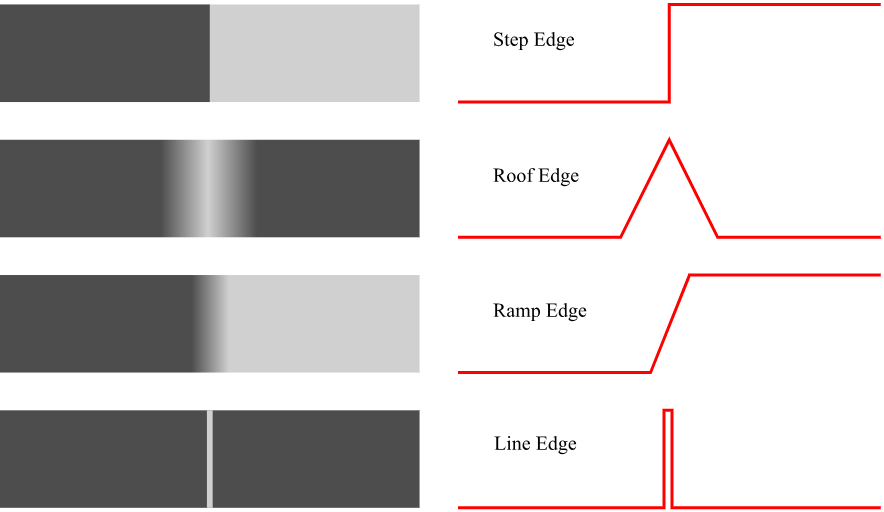
\includegraphics[width=\textwidth]{figures/figure02.png}
    \caption[The 4 common types of edges]{\centering The 4 common types of edges. The left side gives a gives a visual representation of an edge while the right side shows the edge's intensity profile.}
    \label{fig:The 4 common types of edges}
\end{figure}

Having established the definition of an edge, a mathematical way to detect them can be formed.

\section{The Discrete Derivative}
Recall that the definition of the derivative for a differentiable function is given by:
\begin{equation}
    \frac{df}{dx} = \lim_{h \to 0}{\frac{f(x+h) - f(x)}{h}}
\end{equation}
However, it is also useful to know that:
\begin{equation}
    \frac{df}{dx} = \lim_{h \to 0}{\frac{f(x+h) - f(x)}{h} = \lim_{h \to 0}{\frac{f(x) - f(x-h)}{h}} = \lim_{h \to 0}{\frac{f(x+h) - f(x-h)}{2h}}}
    \label{eqn:triple derivative}
\end{equation}

\newpage

Now consider the image intensity profile $I[x]$, a discrete function such that $\{I:I \in \mathbb{Z}, 0 \le I \le 255\}$ and $\{x:x \in \mathbb{Z}, 0 \ge 0\}$ where $I[x]$ denotes the image intensity at pixel $x$. Given the image below:

\begin{figure}[!hbtp]
    \centering
    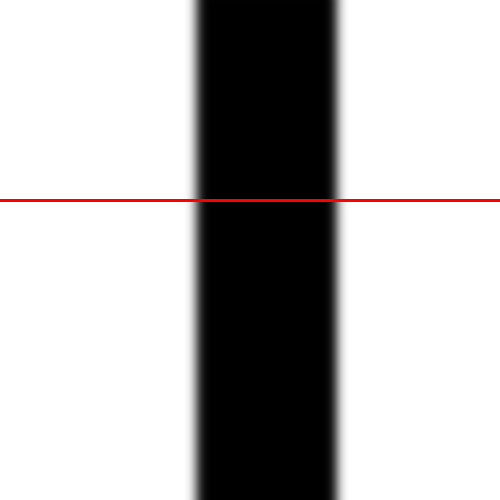
\includegraphics[width=0.5\textwidth]{figures/figure03.png}
    \caption[The intensity profile of this image is denoted by the red line]{\centering The intensity profile of this image is denoted by the red line}
    \label{fig:The intensity profile of this image is denoted by the red line}
\end{figure}

The following graphs can be made:
\begin{figure}[!hbtp]
    \centering
    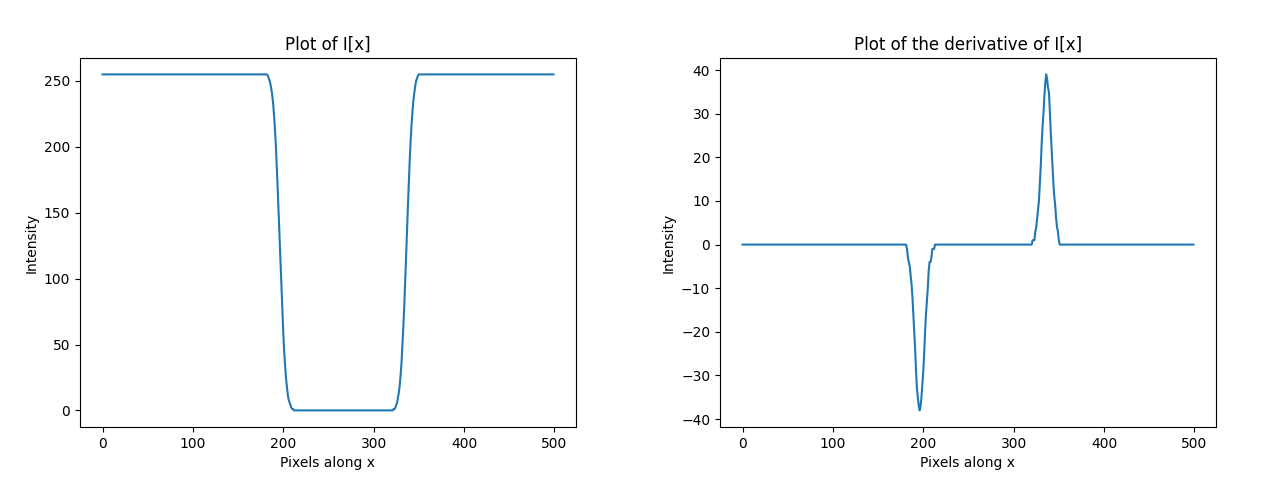
\includegraphics[width=\textwidth]{figures/figure04.png}
    \caption[{Graphs for $I[x]$ and the derivative of $I[x]$}]{\centering Graphs for $I[x]$ and the derivative of $I[x]$}
    \label{fig:Graphs for $I[x]$ and the derivative of $I[x]$}
\end{figure}
Since an edge is defined as a sharp change in image intensity, taking the derivative of $I[x]$
effectively determines the location of edges. To take the derivative of the discrete function $I[x]$,
 the definition
\begin{equation*}
    \frac{dI}{dx} = \lim_{h \to 0}{\frac{f(x+h) - f(x)}{h} = \lim_{h \to 0}{\frac{f(x) - f(x-h)}{h}} = \lim_{h \to 0}{\frac{f(x+h) - f(x-h)}{2h}}}
\end{equation*}
can be rewritten as:
\begin{equation}
    \frac{dI}{dx} = \lim_{h \to 1}{\frac{f[x+h] - f[x]}{h} = \lim_{h \to 1}{\frac{f[x] - f[x-h]}{h}} = \lim_{h \to 1}{\frac{f[x+h] - f[x-h]}{2h}}}
\end{equation}

\end{document}

